\chapter{HASIL DAN PEMBAHASAN}
\section{Hasil Perancangan Sistem}
Sistem deteksi kecacatan kontainer ini dirancang secara otomatis
menggunakan kamera sebagai sensor utama dan lengan robot sebagai
aktuator. Proses diawali dengan model YOLO yang mengidentifikasi
keberadaan kontainer dari input kamera. Jika kontainer terdeteksi,
citra akan dianalisis oleh model Autoencoder untuk mengklasifikasikan
adanya kecacatan. Berdasarkan hasil klasifikasi tersebut, lengan
robot yang digerakkan servo akan menyortir kontainer ke dalam
kategori cacat atau non-cacat. Secara terpisah, sensor PIR
(\textit{Passive Infrared}) berfungsi menghitung jumlah total
kontainer pada setiap kategori, di mana data tersebut kemudian
dikirim (POST) ke server untuk visualisasi pada sisi klien. Desain
sistem yang dirancang diilustrasikan pada Gambar x.

\vspace{1em}

\section{Hasil Perancangan Model YOLO}
\subsection{Dataset dan \textit{Preprocessing}}
Tahap awal dalam penelitian ini adalah pengumpulan data primer berupa
citra kontainer menggunakan kamera. Proses akuisisi data dilakukan
untuk membangun sebuah dataset kustom yang merepresentasikan objek
target secara akurat. Total gambar mentah yang berhasil dikumpulkan
adalah 463 citra. Pengambilan gambar dilakukan dengan melakukan
variasi terhadap lokasi kontainer untuk memastikan model yang akan
dilatih nantinya mampu mengenali objek dengan baik. Dataset kemudian
dibagi menjadi 395 gambar untuk dataset latih dan 68 dataset
validasi. Distribusi pembagian dataset disajikan pada Tabel
\ref{tab:pembagian-dataset}.

\begin{table}[H]
  \caption{Distribusi pembagian dataset}
  \label{tab:pembagian-dataset}
  \vspace{-1em}
  \centering
  \begin{tabular}{ccc}
    \toprule
    \textbf{Kategori} & \textbf{Jumlah Gambar} & \textbf{Persentase} \\
    \midrule
    Data Latih & 395 & 85,3\% \\
    Data Validasi & 68 & 14,7\% \\
    Total Data & 463 & 100\% \\
    \bottomrule
  \end{tabular}
\end{table}

Setelah tahap akuisisi data, proses selanjutnya adalah anotasi
gambar. Anotasi merupakan proses fundamental untuk menghasilkan
dataset berlabel (\textit{labeled dataset}) yang akan digunakan
sebagai data pelatihan (\textit{training data}) [19]. Dalam konteks penelitian
ini, anotasi dilakukan dengan memberikan \textit{bounding box} serta label
kelas pada setiap objek di dalam gambar. Metode ini sangat penting
karena arsitektur YOLO dirancang untuk memprediksi \textit{bounding box} dan
probabilitas kelas secara bersamaan, sehingga memerlukan data latih
dengan format spesifik tersebut untuk dapat melakukan deteksi objek
secara real-time [20]. Sebanyak 463 gambar kontainer telah dianotasi
secara manual. Contoh hasil anotasi dapat dilihat pada Gambar x.

\vspace{1em}

\subsection{Hasil Pelatihan Model}
Pada penelitian ini, mean Average Precision (mAP) digunakan sebagai
metrik utama untuk mengukur performa model YOLO dalam mendeteksi
kontainer kimia. Akurasi deteksi ini sangat penting agar lengan robot
dapat melakukan inspeksi kecacatan secara tepat. Metrik ini dihitung
berdasarkan Average Precision (AP), yang merupakan kombinasi dari
precision dan recall untuk setiap kelas secara individual. Nilai mAP
sendiri adalah rata-rata AP untuk semua kelas, sehingga mampu
memberikan gambaran performa model yang komprehensif [21]. \par

Untuk menentukan apakah sebuah prediksi dianggap benar (true
positive) atau salah (false positive), digunakanlah metrik
Intersection over Union (IoU). IoU merupakan rasio antara area
tumpang tindih (overlap) dari bounding box hasil prediksi
($BB_{predict}$) dengan
bounding box ground truth ($BB_{ground}$), dengan nilai berkisar antara
0 hingga 1 [22].
Semakin mendekati 1, berarti prediksi semakin akurat dan sesuai
dengan objek sebenarnya. IoU dihitung menggunakan persamaan:

\begin{equation}
  IoU = \frac{|BB_{predict} \cap
  BB_{ground}|}{|BB_{predict} \cup BB_{ground}|}
\end{equation}

Precision mengukur proporsi prediksi positif yang benar (True
Positive) terhadap seluruh prediksi positif (TP + False Positive),
sehingga menunjukkan kemampuan model dalam meminimalkan kesalahan
deteksi (false positives). Sementara itu, recall atau true positive
rate mengukur seberapa banyak instance positif sebenarnya yang
berhasil dideteksi dengan benar, sehingga menggambarkan kemampuan
model dalam menemukan semua objek yang ada (minim false negatives)
[23]. Precision dan Recall dapat dihitung menggunakan persamaan:

\begin{equation}
  Precision = \frac{TP}{TP + FP}, \quad
  Recall = \frac{TP}{TP + FN}
\end{equation}

mAP adalah nilai rata-rata dari AP untuk semua kelas. Karena model
YOLO yang digunakan dalam penelitian ini hanya
memprediksi satu kelas yaitu kontainer kimia, maka nilai mAP setara
dengan nilai AP. Nilai AP sendiri dihitung sebagai rata-rata
precision di seluruh
rentang nilai recall (0 hingga 1) [24], sebagaimana dirumuskan dalam
Persamaan 3, di mana P adalah precision dan r adalah recall.

\begin{equation}
  AP = \int_{0}^{1} P(r) \,dr
\end{equation}

Proses pelatihan model YOLO dilakukan menggunakan platform Google
Colaboratory. Model dilatih secara iteratif selama 50 epoch dengan
batch size 16 dan optimizer Adam, agar model dapat mempelajari
fitur-fitur dari data latih secara optimal. Hasil pelatihan model
YOLO setiap 10 epoch dapat dilihat pada Tabel \ref{tab:yolo-train}.

\begin{table}[H]
  \caption{Proses training model YOLO}
  \label{tab:yolo-train}
  \vspace{-1em}
  \centering
  \footnotesize
  \begin{tabular}{c p{1.5cm} p{1.5cm} p{1.5cm} p{1.5cm} p{1.5cm} p{1.5cm}}
    \toprule
    \textbf{Epoch} & \textbf{Train/Box Loss} & \textbf{Train/Class Loss}
    & \textbf{Train/DFL Loss} & \textbf{Val/Box Loss}
    & \textbf{Val/Class Loss} & \textbf{Val/DFL Loss} \\
    \midrule
    0 & 0.59460 & 1.93744 & 0.97064 & 0.47086 & 2.50286 & 0.89899 \\
    10 & 0.43332 & 0.43561 & 0.87133 & 0.30517 & 0.37575 & 0.82624 \\
    20 & 0.32857 & 0.29349 & 0.85098 & 0.33417 & 0.21048 & 0.84483 \\
    30 & 0.28212 & 0.23284 & 0.83904 & 0.24181 & 0.15662 & 0.82436 \\
    40 & 0.22672 & 0.17762 & 0.80096 & 0.22091 & 0.13860 & 0.82009 \\
    50 & 0.20164 & 0.15458 & 0.79927 & 0.20030 & 0.11625 & 0.81561 \\
    \bottomrule
  \end{tabular}
  \normalsize
\end{table}

Pada proses training, nilai loss pada data train dan validasi secara
umum menunjukkan tren penurunan seiring bertambahnya epoch. Penurunan
ini menunjukkan bahwa model semakin mampu menyesuaikan parameter
internalnya dengan data yang diberikan. Dengan demikian, model
menjadi lebih baik dalam mempelajari pola yang relevan untuk
mendeteksi kontaier.

Pada Train/Box Loss, terjadi penurunan signifikan dari 0.59460 pada
epoch ke-0 menjadi 0.20164 pada epoch ke-50, yang mengindikasikan
peningkatan kemampuan model dalam memprediksi posisi bounding box
secara lebih akurat. Hal serupa juga terlihat pada Train/Class Loss,
yang turun drastis dari 1.93744 menjadi 0.15458, menandakan model
semakin tepat dalam melakukan klasifikasi objek. Sementara itu,
Train/DFL Loss (Distribution Focal Loss) menurun dari 0.97064 menjadi
0.79927, yang berarti model semakin baik dalam memperbaiki distribusi
prediksi bounding box. Pada data validasi, Val/Box Loss menurun dari
0.47086 ke 0.20030, Val/Class Loss dari 2.50286 ke 0.11625, serta
Val/DFL Loss dari 0.89899 ke 0.81561. Penurunan yang konsisten pada
semua komponen loss validasi menunjukkan bahwa model tidak hanya
mampu belajar dengan baik pada data train, tetapi juga memiliki
kemampuan generalisasi yang baik terhadap data yang belum pernah
dilihat sebelumnya.

Namun, evaluasi kinerja model tidak bisa hanya mengandalkan nilai
loss. Perlu digunakan metrik tambahan seperti mAP  untuk menilai
akurasi deteksi dan kualitas prediksi bounding box secarah
menyeluruh. Pada penelitian ini digunakan mAP@50 (IoU threshold 50\%)
untuk mengukur keberhasilan deteksi secara lebih longgar, serta
mAP@95 (rata-rata mAP dari IoU threshold 50\% hingga 95\% dengan
interval 5\%) untuk menilai ketepatan prediksi bounding box secara
lebih ketat dan detail. Hasil pengukuran mAP pada tiap epoch dapat
dilihat pada Gambar \ref{fig:map}.

\begin{figure}[H]
  \centering
  % First image
  \begin{minipage}[t]{0.48\textwidth}
    \centering
    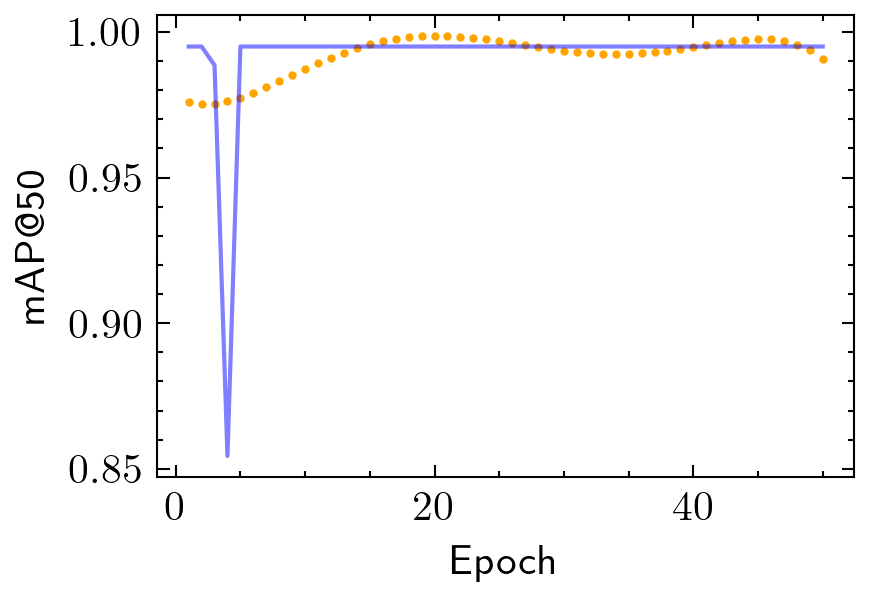
\includegraphics[width=\textwidth]{gambar/map50.png}
    (a)
  \end{minipage}
  \hfill
  % Second image
  \begin{minipage}[t]{0.48\textwidth}
    \centering
    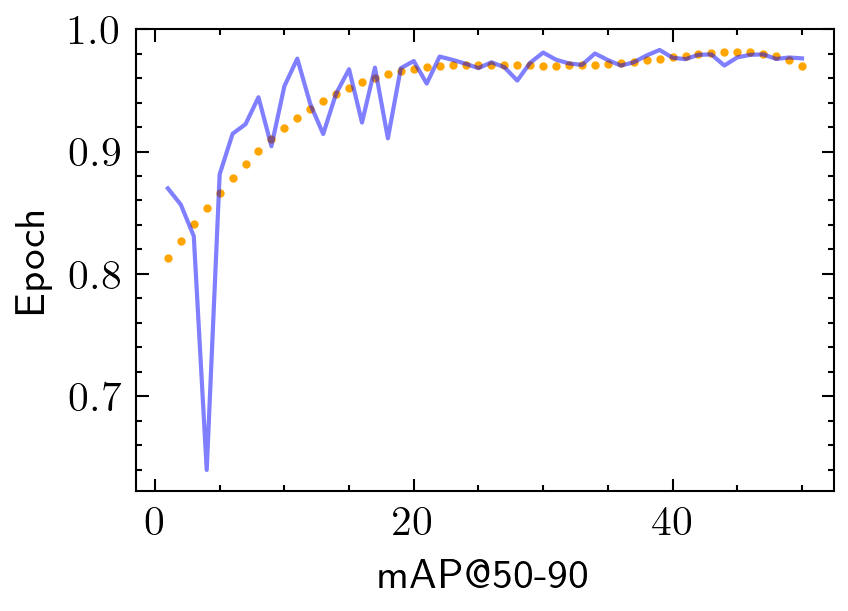
\includegraphics[width=\textwidth]{gambar/map5090.png}
    (b)
  \end{minipage}
  \caption{Grafik tren mAP: (a) mAP@50, (b) mAP@50-90}
  \label{fig:map}
  \vspace{-1em}
\end{figure}

Grafik tersebut menyajikan evaluasi performa model deteksi objek
menggunakan metrik mean Average Precision (mAP) seiring berjalannya
50 epoch pelatihan. Grafik di sebelah kiri, mAP@50, yang menggunakan
ambang batas IoU longgar (50\%), menunjukkan bahwa model dengan
sangat cepat mencapai performa puncak. Terlihat bahwa nilainya
melonjak mendekati 1.00 hanya dalam 10-15 epoch pertama lalu
cenderung datar, menandakan model mampu mempelajari cara mendeteksi
keberadaan objek secara umum dengan sangat cepat. Sebaliknya, grafik
di sebelah kanan, mAP@50-95, yang mengukur performa pada rentang
ambang batas IoU yang lebih ketat (50\% hingga 95\%), menunjukkan
kurva pembelajaran yang lebih bertahap dan konsisten. Peningkatan
yang lebih landai ini mengindikasikan bahwa model menggunakan
mayoritas waktu pelatihannya untuk terus-menerus menyempurnakan
presisi dan akurasi lokalisasi bounding box-nya. Secara keseluruhan,
pencapaian nilai mAP yang sangat tinggi pada kedua metrik di akhir
pelatihan menandakan model final yang dihasilkan tidak hanya mampu
mendeteksi objek, tetapi juga sangat akurat dalam menentukan
batas-batasnya. Hasil deteksi kontainer kimia pada data validasi
dapat dilihat pada Gambar \ref{fig:yolo-validasi}.

\begin{figure}[H]
  \centering
  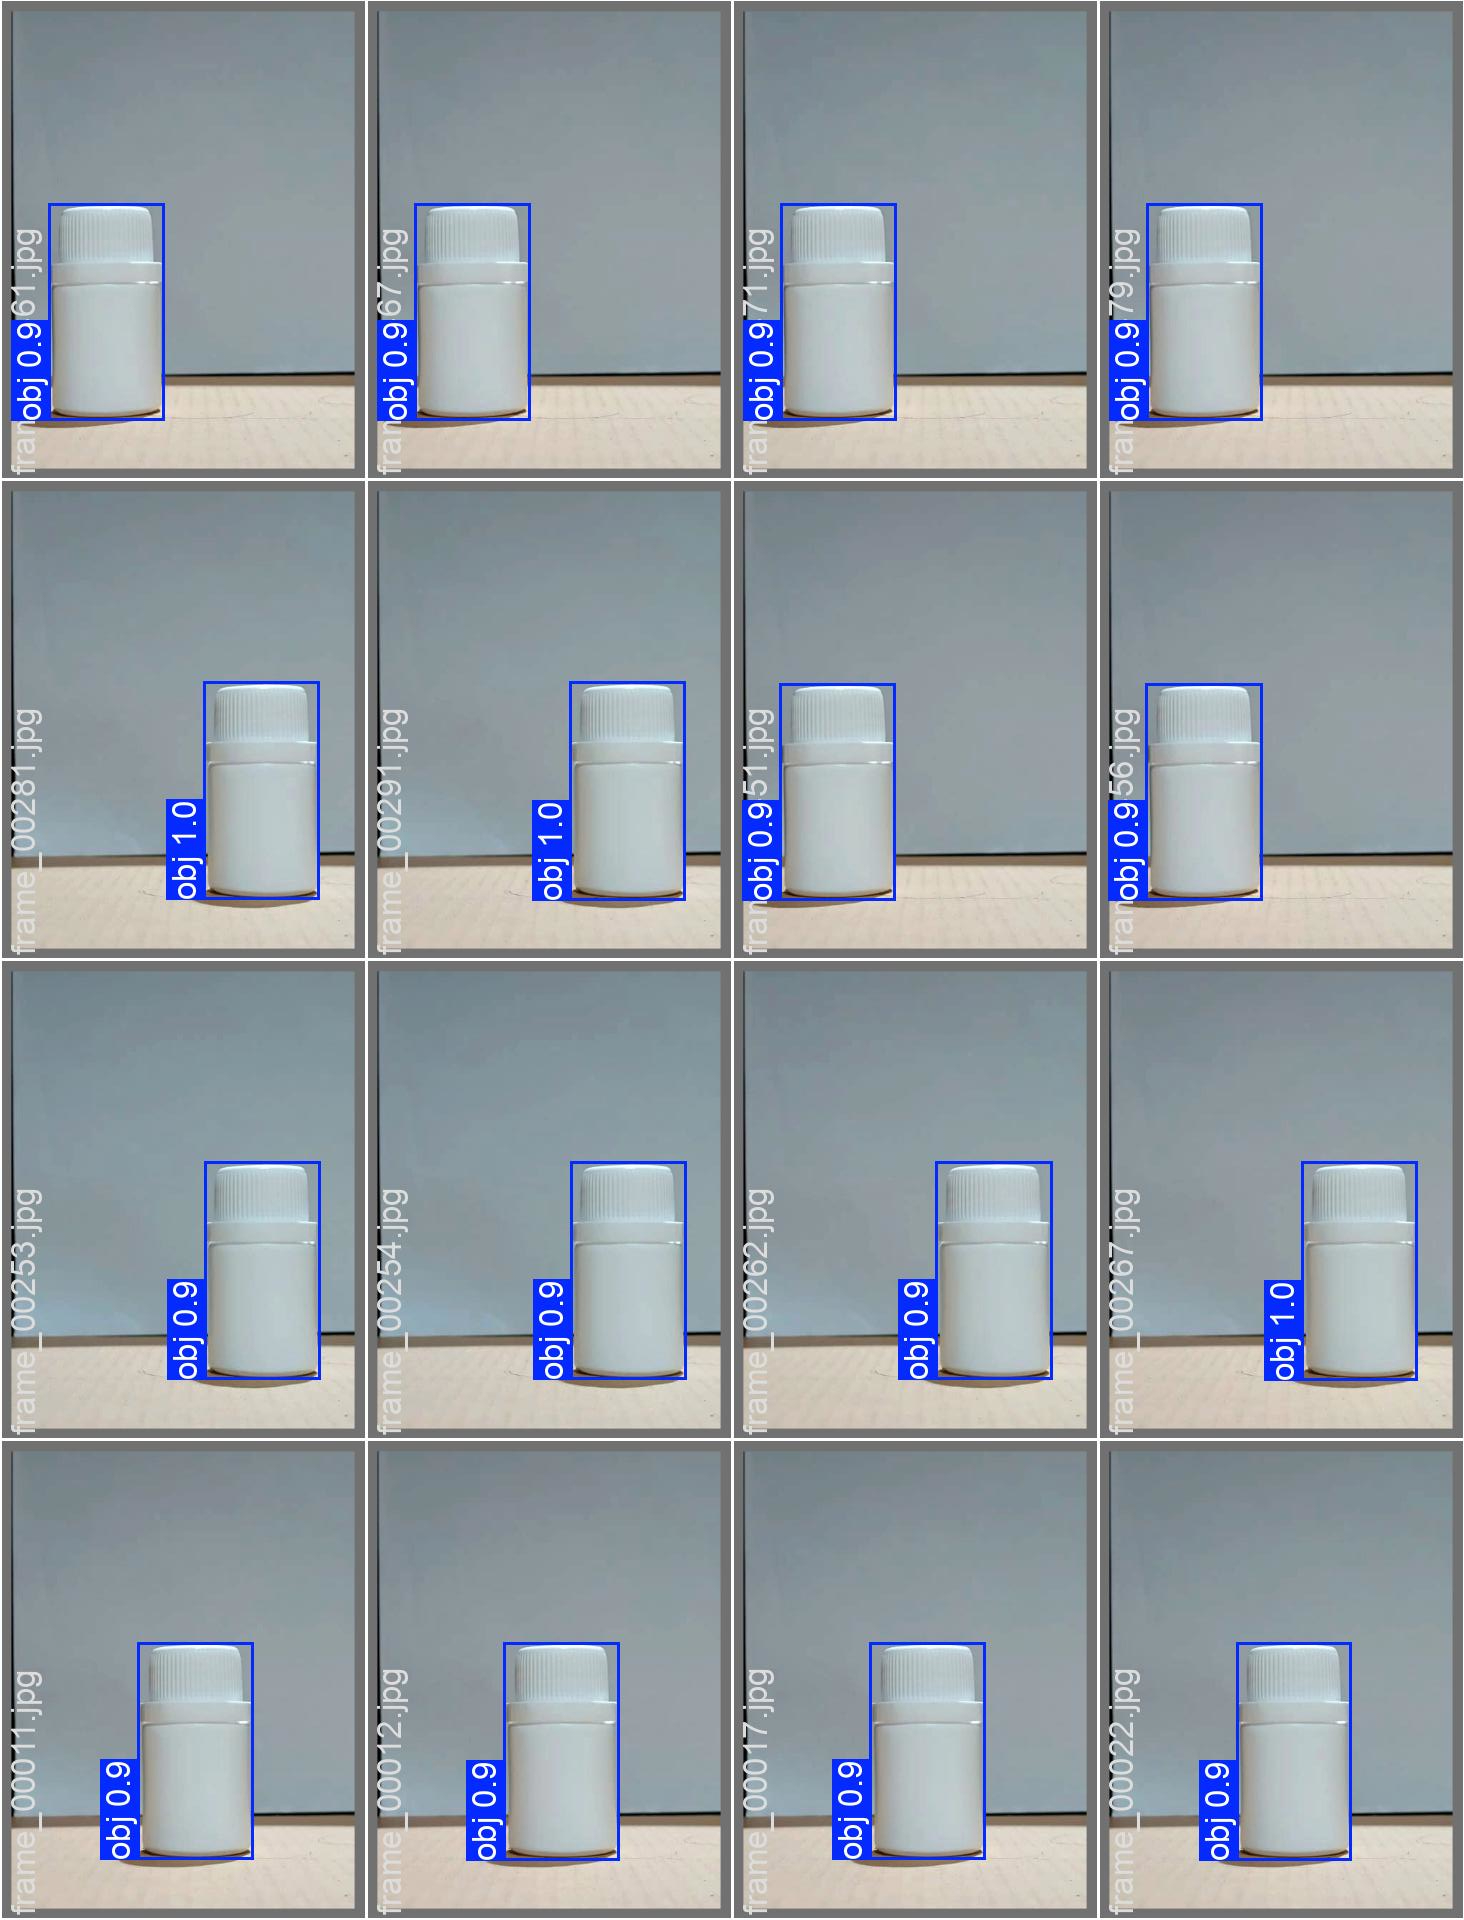
\includegraphics[width=0.7\textwidth]{gambar/yolo_validasi.jpg}
  \caption{Hasil prediksi YOLO pada data validasi}
  \label{fig:yolo-validasi}
\end{figure}
\vspace{-1em}

\vspace{1em}

\section{Hasil Perancangan Model Deteksi Kecacatan}
\subsection{Arsitektur Variational Autoencoder}
\subsection{Hasil Rekonstruksi dan Error}
\subsection{Penentuan Threshold Kecacatan}

\vspace{1em}

\section{Hasil Pengujian Sistem}
